\documentclass[10pt]{article}

   \addtolength{\oddsidemargin} {-0.9in}
   \addtolength{\textwidth}{1.7in}
   \addtolength{\topmargin}{-1.2in}
   \addtolength{\textheight}{2in}
   \linespread{1.1}
   \usepackage{graphicx}
   \usepackage{fancyhdr}
   \usepackage{url}
   \usepackage{amsmath,amssymb}
   \usepackage{comment}
   \usepackage{float}
   \pagestyle{fancy}
\lhead{} \chead{} \rhead{} \cfoot{} \rfoot{\thepage}
\renewcommand{\headrulewidth}{0.0pt}
\renewcommand{\footrulewidth}{0.4pt}
\usepackage{xcolor}
\definecolor{mygray}{gray}{0.9}
\usepackage[colorlinks=true,linkcolor=blue,citecolor=blue,urlcolor=blue]{hyperref}
\usepackage{chemmacros}

\usepackage{listings}
\usepackage{color} %red, green, blue, yellow, cyan, magenta, black, white
\definecolor{mygreen}{RGB}{28,172,0} % color values Red, Green, Blue
\definecolor{mylilas}{RGB}{170,55,241}

\lstset{language=Matlab,%
    breaklines=true,%
    morekeywords={matlab2tikz},
    keywordstyle=\color{blue},%
    morekeywords=[2]{1}, keywordstyle=[2]{\color{black}},
    identifierstyle=\color{black},%
    stringstyle=\color{mylilas},
    commentstyle=\color{mygreen},%
    showstringspaces=false,%without this there will be a symbol in the places where there is a space
    numbers=left,%
    numberstyle={\tiny \color{black}},% size of the numbers
    numbersep=9pt, % this defines how far the numbers are from the text
    emph=[1]{for,end,break},emphstyle=[1]\color{red}, %some words to emphasise
}

\begin{document}

\begin{center}
{\Large\bf Homework \#8}\\
 {\bf Name: Andrea Livingston}\\
 {\bf Due: November 11th, 2016}\\
 {\bf CBE660: Intermediate Problems in Chemical and Biological
Engineering\; -\; Fall 2016}\\
Department of Chemical and Biological Engineering, University of Wisconsin-Madison
\end{center}

\noindent\colorbox{mygray}{\begin{minipage}{\textwidth}
  {\bf Problem 1}. Solve problem 2.5 in the textbook and show that the Fourier series $f(x)=\sum_{k=-K}^Kc_ke^{ikx}$ can be expressed as $f(x)=a_0+\sum_{k=1}^K\left(a_k\cos(kx)+b_k\sin(kx)\right)$. How are the coefficients $c_k$ related to $a_0,a_k,b_k$?
\end{minipage}}
\\

{\em Solution:}   
\\
\\
We can show that the expressions are equivalent by showing that $c_k=\bar{c}_{-k}$
\[c_k=\frac{(f,e^{ikx})}{e^{ikx},e^{ikx}}=\frac{(f,e_k)}{(e_k,e_k)} \]
\[c_{-k}=\frac{(f,e^{-ikx})}{e^{-ikx},e^{-ikx}}\]
\\
Finding the complex conjugate for $c_{-k}$
\[\bar{c}_{-k}=\frac{(f,e^{ikx})}{e^{ikx},e^{ikx}}\]
Because this expression for $\bar{c}_{-k}$ is equivalent to the expression for $c_k$, the expressions for f(x) are equivalent. 
\\
\\
Thus,
\[ \sum_{k=-K}^Kc_ke^{ikx}=a_0+\sum_{k=1}^K\left(a_k\cos(kx)+b_k\sin(kx)\right)\]
From inspection, we can see that $a_0=c_0$. Now relating $a_k$ and $b_k$ to $c_n$.
\\
Consider the signals that oscillate once in a period (k=1)
\[ c_{-1}e^{-ix}+c_{1}e^{ix}=a_1cos(x) +b_1sin(x) \]
\\
And then for two oscillations in a single period (k=2)
\[ c_{-2}e^{-2ix}+c_{2}e^{2ix}=a_2cos(2x) +b_2sin(2x) \]
Generalizing this relationship, we can say
\[ c_ke^{kix}+c_{-k}e^{-kix}=a_kcos(kx)+b_ksin(kx) \]
\\
Given that f(x) is a real function and that $e^{-kix}$ is the complex conjugate of $e^{kix}$, we can say that $c_{-k}$ is the complex conjugate of $c_k$. This allows the complex terms to cancel out from the exponential expression, such that the final expression is entirely real. $c_k=Re(c_k)+Im(c_k)$ and $\bar{c}_k=Re(c_k)-Im(c_k)$
\[ c_ke^{kix}+c_{-k}e^{-kix}=a_kcos(kx)+b_ksin(kx) \]
\[ c_ke^{kix}+c_{-k}e^{-kix} = (Re(c_k)-j*Im(c_k))(cos(kx)-jsin(kx)+(Re(c_k)+j*Im(c_k))(cos(kx)+j*sin(kx))\]
Distributing the terms and simplifying yeilds
\[c_ke^{kix}+c_{-k}e^{-kix} = 2*Re(c_k)cos(kx)-2*Im(c_k)sin(kx)  \]
Substituting back into the exponential side of the original expression
\[ 2*Re(c_k)cos(kx)-2*Im(c_k)sin(kx)  = a_kcos(kx)+b_ksin(kx)\]
Using this, $2*Re(c_k) = a_k$ and $-2*Im(c_k)=b_k$
Relating this back to $c_k$
\[ c_k=\frac{a_k}{2}-j*\frac{b_k}{2} \]

\newpage

\noindent\colorbox{mygray}{\begin{minipage}{\textwidth}
  {\bf Problem 2}. Use a Fourier series to approximate the Gaussian kernel function $f(x)=\exp(-ax^2)$ with $a\geq 0$ and $x\in [-L,L]$. Develop Matlab code to approximate the function for $L=1$ and $a=0,2,4,8$. Plot the error of the approximation as a function of $K$. What order of convergence do you observe?
  \end{minipage}}
\\

{\em Solution:}   
\\
\\
The Fourier series for the Gaussian Kernel Function $f(x)=exp(-ax^2)$ with $a\geq 0$ and $x\epsilon[-L,L]$
\[f(x)=exp(-ax^2)=\sum_{k=-\infty}^{\infty}c_ke^{ikx} \]
\[ c_k=\frac{1}{2\pi}\int_{-\pi}^{\pi}f(x)e^{-ikx}dx \]
\\
To change the boundaries from $\pi$ to $L$, now $x=x\frac{\pi}{L}$
\[ c_k=\frac{1}{2L}\int_{-L}^{L}e^{-a(x \frac{\pi}{L})^2}e^{-ikx\frac{\pi}{L}} \]
Substituting $e^{-ikx}=cos(kx)-i*sin(kx)$
\[ c_k=\frac{1}{2L}\int_{-L}^{L}e^{-a(x \frac{\pi}{L})^2} \left(cos(-kx\frac{\pi}{L})-i*sin(kx\frac{\pi}{L})\right) \]
\[ c_k=\frac{1}{2L}\int_{-L}^{L}e^{-a(x \frac{\pi}{L})^2} cos(kx\frac{\pi}{L})-\frac{1}{2L}\int_{-L}^{L}e^{-a(x \frac{\pi}{L})^2}i*sin(kx\frac{\pi}{L}) \]
The sin function is an odd function such that the integral of sin will be zero. The positive area of the sin curve plus the negative area of the sin curve will go to zero when summed. Although the Gaussian function is an even function, an even function times an odd function will still yield an odd function. Thus, the second term goes to zero when integrated.

\[ c_k=\frac{1}{2L}\int_{-L}^{L}e^{-a(x \frac{\pi}{L})^2} cos(kx\frac{\pi}{L}) \]
While this integral can be analytically determined, it is easiest to approximate the integral as $x\epsilon[-\infty,\infty]$ so that it represents a standard integral. 

\[ \int_{-\infty}^{\infty}e^{\frac{-x^2}{\sigma^2}}cos(\beta x)dx= \sqrt{\pi}\sigma e^{\frac{-\beta^2\sigma^2}{4}}\]
Using this standard integral approximation $\frac{1}{\sigma^2}=a(\frac{\pi}{L})^2$ and $\beta = k\frac{\pi}{L}$. 

\[ \sigma=\frac{L}{\pi}\sqrt{\frac{1}{a}} \]

\[ c_k=\frac{1}{2L}\sqrt{\pi}\sigma exp\left[ -(\frac{\beta\sigma}{2})^2   \right] \]

\[ c_k=\frac{1}{2}\sqrt{\frac{\pi}{a}}exp\left[ \frac{-k^2\pi^2}{4a} \right] \]
\\
Returning to the original series

\[f(x)=e^{-ax^2}=\sum_{k=-\infty}^{\infty}c_ke^{\frac{ikx\pi}{L}} \]

\[f(x)=exp(-ax^2)=\sum_{k=-\infty}^{\infty} \left(\frac{1}{2}\sqrt{\frac{\pi}{a}}exp\left[ \frac{-k^2\pi^2}{4a} \right] \right) e^{\frac{ikx\pi}{L}} \]

\[ f(x)=\frac{1}{2}\sqrt{\frac{\pi}{a}} \sum_{k=-\infty}^{\infty} exp\left[ \frac{-k^2 \pi^2}{4a} \right] e^{\frac{ikx\pi}{L}} \]
\\
This can be approximated by truncating the summation from $[-\infty,\infty]$ to $[-c,c]$

\[ f(x) \approx \frac{1}{2}\sqrt{\frac{\pi}{a}} \sum_{k=-c}^{c} exp\left[ \frac{-k^2 \pi^2}{4a} \right] e^{\frac{ikx\pi}{L}} \]
\\
Comparing the approximation to Gaussian distribution we can see that the fit improves as a increases (the lines are stacked). The fit with a=0 was approximated with a very small value for a to avoid dividing by a zero. However, dividing by a small number gives a very large result for the approximation. 

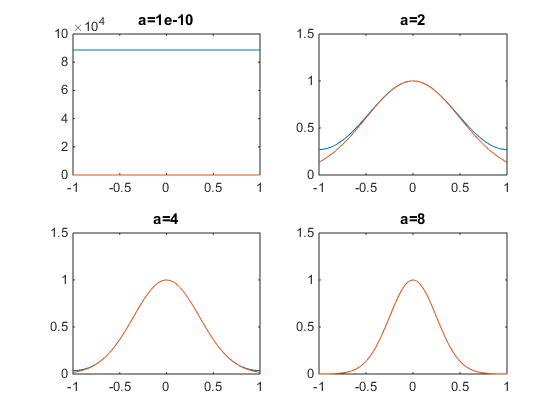
\includegraphics{CBE660_Assign8_2_Fig2.png} \\
\\
As a result of the approximation for a=0, the error results were not meaningful. For the others, it can be seen that the error decreases as a increases. 

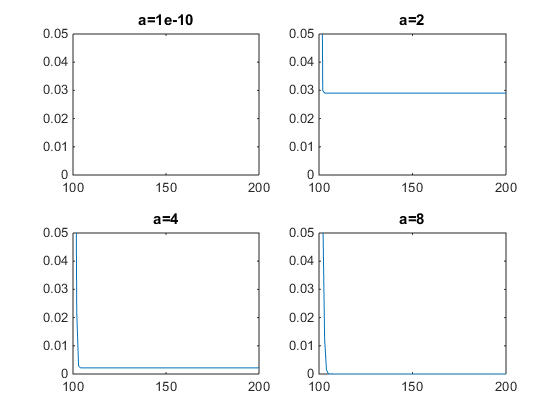
\includegraphics{CBE660_Assign8_2_Fig1.png} \\

\lstinputlisting{CBE660_Assign8_2.m}



\newpage

\noindent\colorbox{mygray}{\begin{minipage}{\textwidth}
  {\bf Problem 3}.  Electrical loads of consumers are quasi-periodic and notoriously difficult to satisfy by the power grid because they vary over a wide range of frequencies. Think about how your electricity demands at home vary daily, hourly, and within seconds due to natural human behavior and fast equipment fluctuations (e.g., your fridge). Similar multi-scale behavior is observed in systems that might seem static to the human eye but in which high-frequency effects exist.  Assume that you have the load in Figure \ref{fig1} and after applying the discrete Fourier transform you obtain the spectrum shown in Figure \ref{fig2}. The spectrum has the components $|\bar{f}(j\omega_0)|=10$ for $\omega_0=0\,Hz$, $|\bar{f}(j\omega_1)|=5$ for $\omega_1=1.1574\times 10^{-5}\,Hz$, $|\bar{f}(j\omega_2)|=2.5$ for $\omega_2=2.3148\times 10^{-5}\,Hz$, and $|\bar{f}(j\omega_3)|=0.5$ for $\omega_3=3.7037\times 10^{-4}\, Hz$.  Answer the following:
  
  \begin{itemize}
  \item What are time-domain functions $f_0(t),f_1(t),f_2(t),f_3(t)$ that, when combined as $f(t)=f_0(t)+f_1(t)+f_2(t)+f_3(t)$, give rise to the load $f(t)$? 
  \item Verify that the sum of your functions matches the load data provided.
  \item For each $\omega_k,\, k=0,1,2,3$ determine the number of cycles per day for the load component $f_k(t)$ (i.e., how many times in a day does $f_k(t)$ crosses zero). 
  \end{itemize}
  \end{minipage}}
\\

\begin{figure}[!htb]
\begin{center}
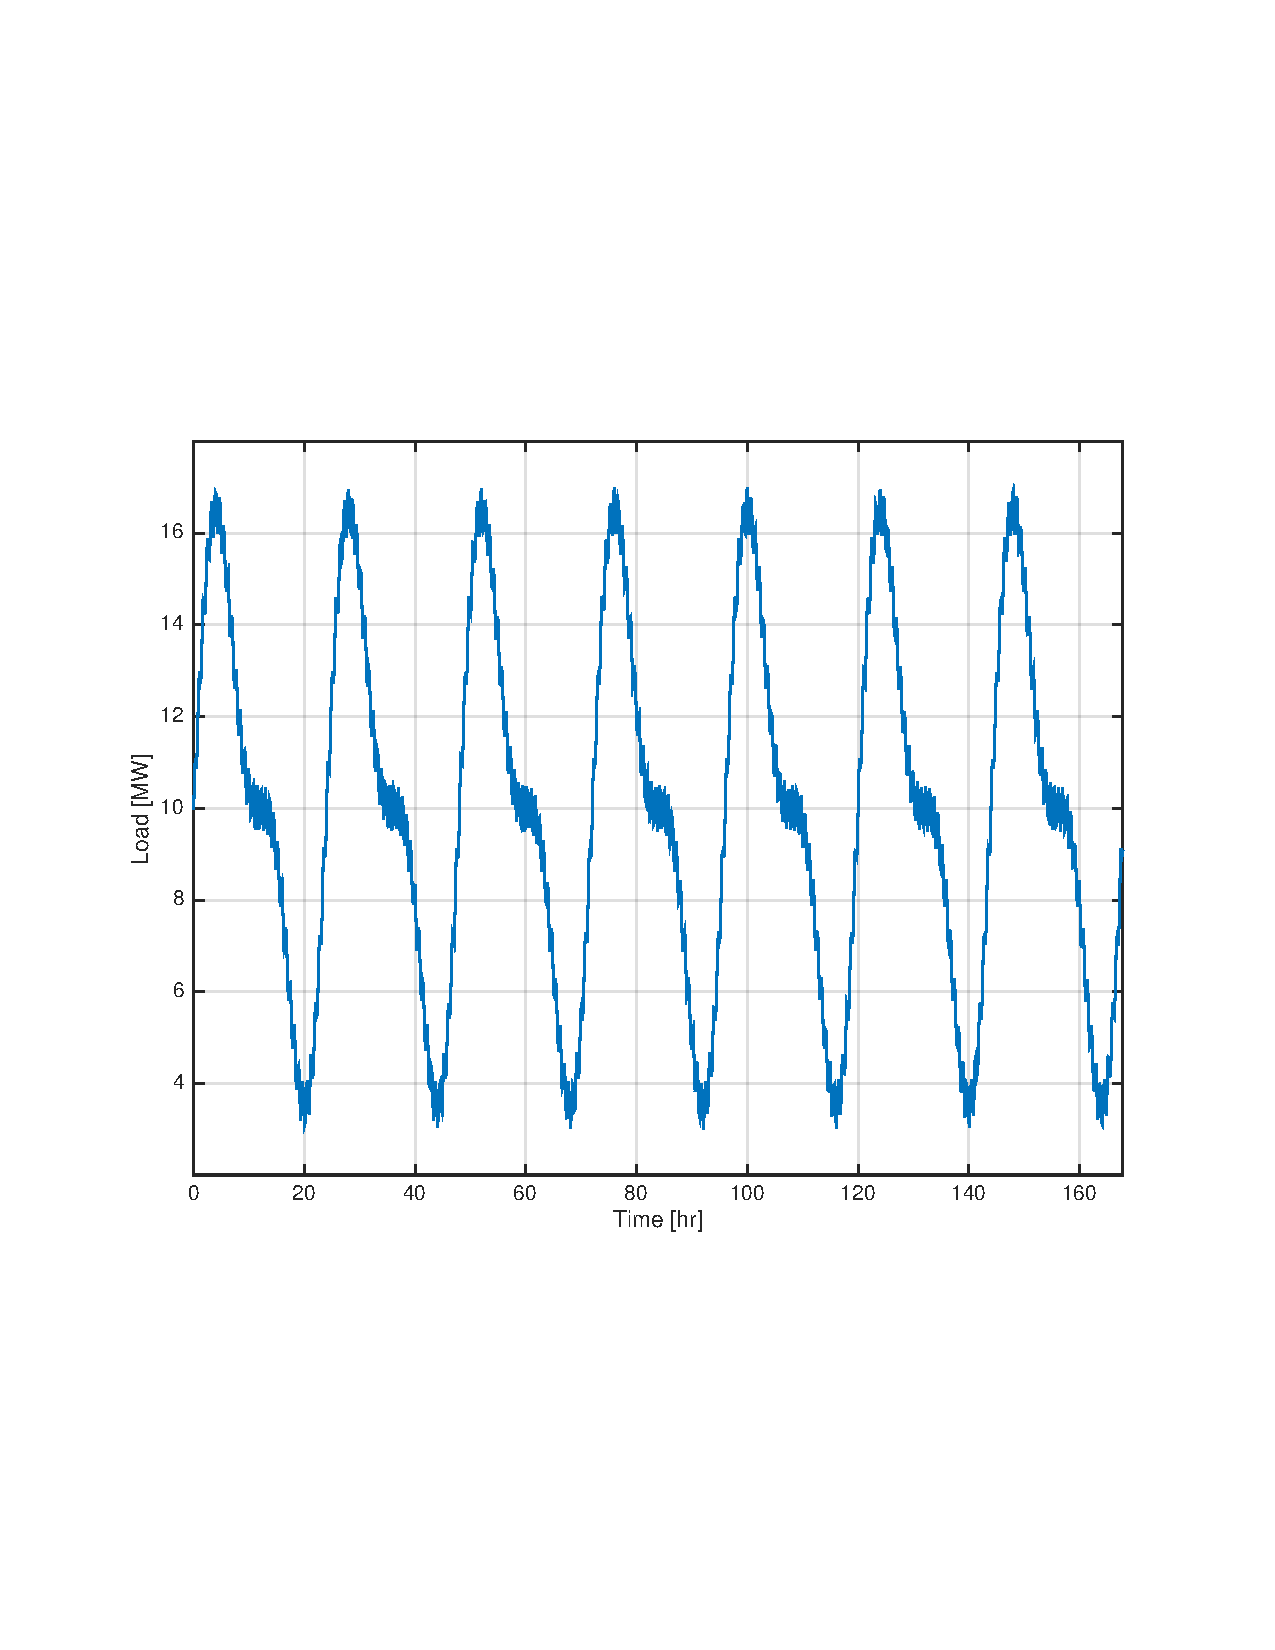
\includegraphics[width=3in]{CBE660_HW8_file1.pdf}\caption{Electrical load.}\label{fig1}
\end{center}
\end{figure}


\begin{figure}[!htb]
\begin{center}
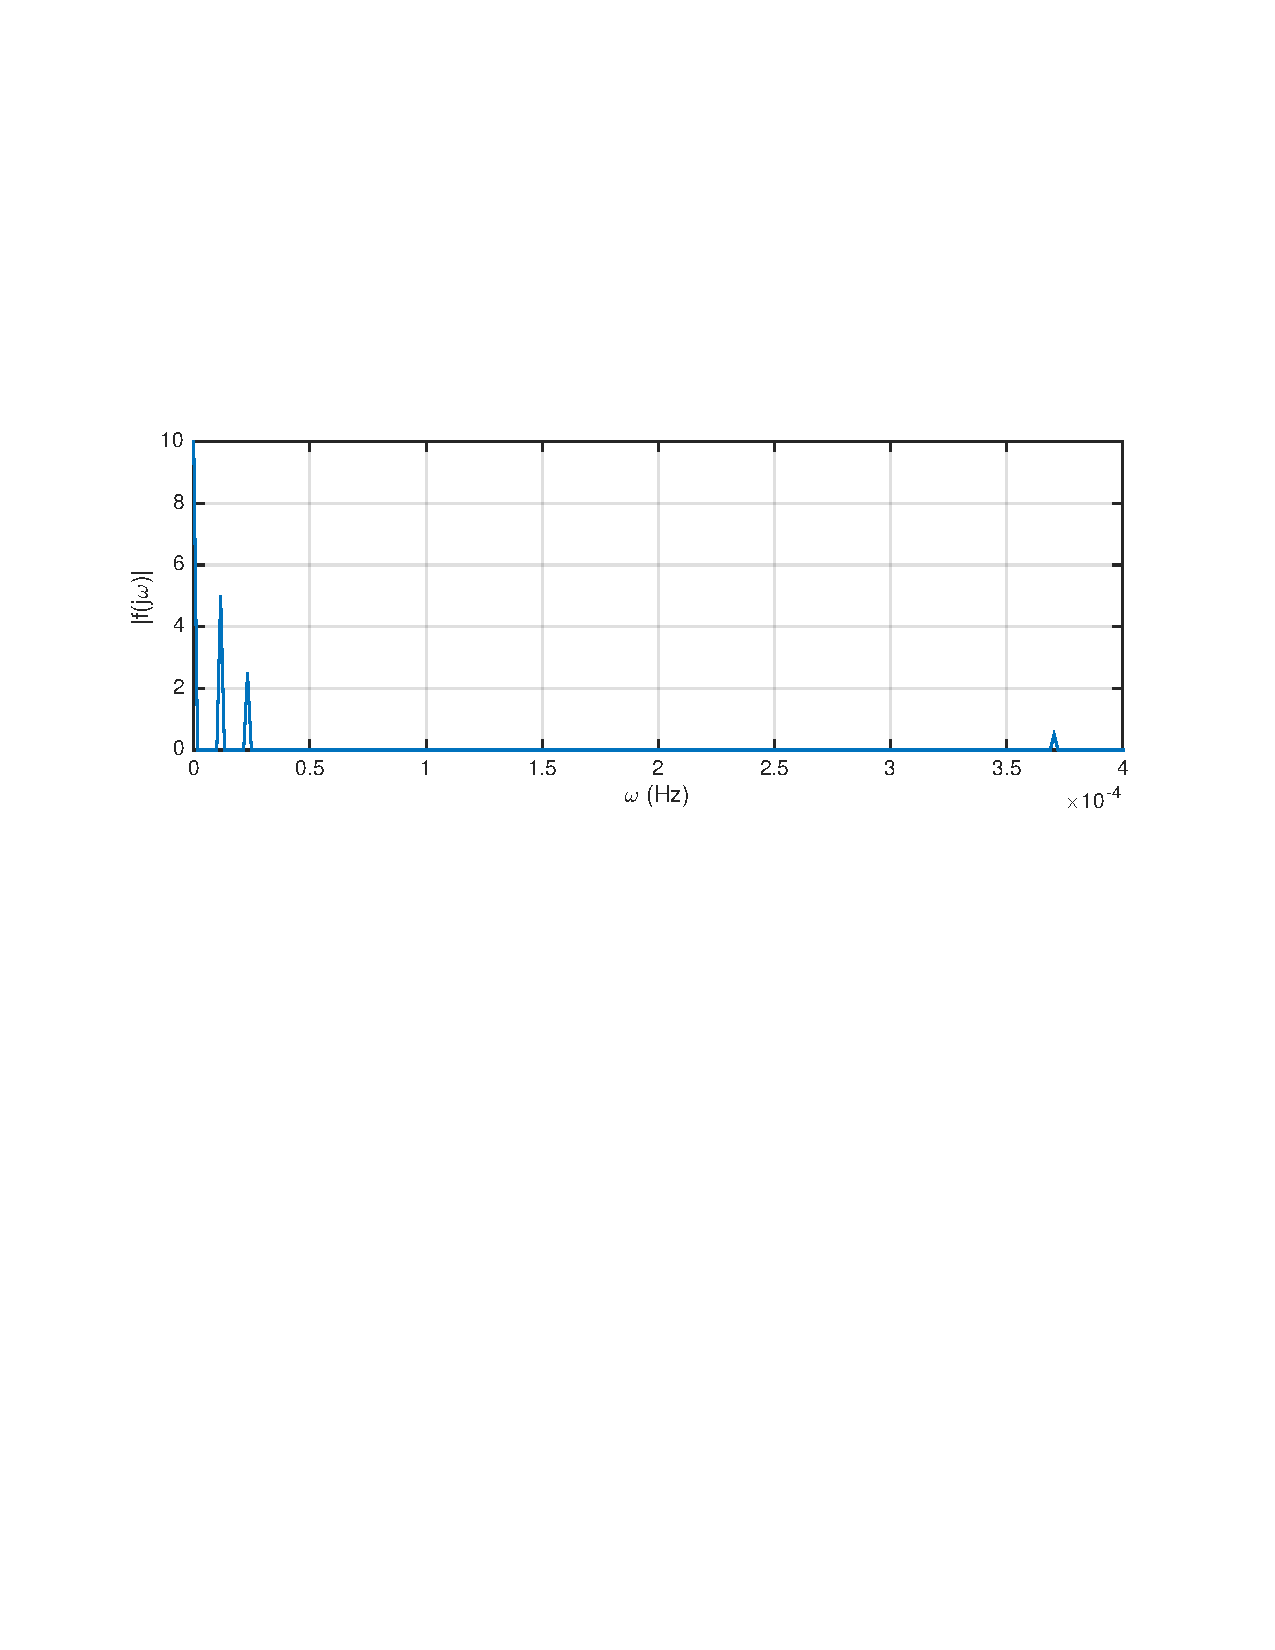
\includegraphics[width=5in]{CBE660_HW8_file2.pdf}\caption{Fourier spectrum of electrical load.}\label{fig2}
\end{center}
\end{figure}


{\em Solution:}   
\\
\\
The statement begins in the Fourier domain and we need to move back into the time domain. We can do this  by taking the Inverse Fourier Transform. 
\[f(t)=\int_{-\infty}^{\infty}F(k)e^{2\pi j\omega t} d\omega \]
\\
Developing an expression for $F(k)$ from the provided information
\[ F(k)=F(j\omega_0)\delta(\omega-\omega_0)+F(j\omega_1)\delta(\omega-\omega_1)+F(j\omega_2)\delta(\omega-\omega_2)+F(j\omega_3)\delta(\omega-\omega_3)=\sum_{k=0}^{3}F(j\omega_k)\delta(\omega-\omega_k) \]
\\
Substituting this into the inverse Fourier expression
\\
\[ f(t)=\int_{-\infty}^{\infty}\sum_{k=0}^{3}F(j2\pi\omega_k)\delta(2\pi\omega-2\pi \omega_k)e^{2\pi jkt} d\omega\]
\\
Because the summation does not depend on the variable of integration, k, it can be brought outside the integral
\[ f(t)=\sum_{k=0}^{3}F(j2\pi\omega_k)\int_{-\infty}^{\infty}\delta(2\pi(\omega-\omega_k))e^{2\pi jkt} d\omega \]
\\
Then the $2\pi$ cancels out of the delta function
\[ f(t)=\sum_{k=0}^{3}F(j2\pi\omega_k)\int_{-\infty}^{\infty}\delta(\omega-\omega_k)e^{2\pi jkt} d\omega \]
\\
The integral can be evaluated according the the standard integral $\int_{-\infty}^{\infty}f(x)\delta(x-a)=f(a)$ with the integration variable $k$ being replaced by $\omega_k$
\[ f(t)=\sum_{k=0}^{3}F(j2\pi\omega_k)e^{2\pi j \omega_k t} \]
\\
Applying the Euler Identity property to break the exponential into trig functions
\[ e^{2\pi j \omega_k t} = cos(2 \pi \omega_k t)+j*sin(2 \pi \omega_k t) \]
\[ f(t)= \sum_{k=0}^{3}F(j2\pi\omega_k)\left[cos(2 \pi \omega_k t)+j*sin(2 \pi \omega_k t)\right] \]
\\
Pulling the first term out of the summation such that the sum runs from k=1 to k=3 
\[ f(t)=F(2\pi j \omega_0)   \left[cos(2 \pi \omega_0 t)+j*sin(2 \pi \omega_0 t)\right] + \sum_{k=1}^{3}F(j2\pi\omega_k)\left[cos(2 \pi \omega_k t)+j*sin(2 \pi \omega_k t)\right] \]
\\
Now substituting the value of $\omega_0=0$ in to simplify the trigonometric expressions according to $cos(0)=1$ and $sin(0)=0$ 
\[ f(t)=F(2\pi j \omega_0) + \sum_{k=1}^{3}F(j2\pi\omega_k)\left[cos(2 \pi \omega_k t)+j*sin(2 \pi \omega_k t)\right]  \]
\\
Consider figure(1) which is an odd function. An odd function can only be created by summing together all odd functions. From our expression, cos is an even function and sin is an odd function because there is no phase shift. Because figure (2) is comprised \textit{only } of odd functions, we can assume that cos()=0 at all locations of interest, thus reducing the overall expression. 
\[ f(t)=F(2\pi j \omega_0) + \sum_{k=1}^{3}F(j2\pi\omega_k)j*sin(2 \pi \omega_k t) \]
\\
Now, we can see that $F(2 \pi j \omega_k)$ must relate to each of the coefficients $c_k$ in the overall summation. To find their respective values we can consider $|F(2 \pi j \omega_k)|=\left[ Re()^2+Im()^2  \right]^{1/2}$. From figure(1) we can assume that f(t) has only real components in the domain of interest. To cancel with imaginary term from the sin, $F(2 \pi j \omega_k)$ must only contain an imaginary part to make the overall expression real. 
\[ |F(2 \pi j \omega_k)|=[Re()^2+Im()^2]^{1/2} = |Im()| \]
\\
Let $Im()=-|Im()|*j$ such that $F(2\pi j \omega_k)=-j*Im()=-j*|F(j2 \pi \omega_k)|$
\[ f(t)=F(2\pi j \omega_0) + \sum_{k=1}^{3}-|F(j2\pi\omega_k)|*j*j*sin(2 \pi \omega_k t) \]
\\
Now the imaginary components cancel out $(j*j=-1)$
\[ f(t)=F(2\pi j \omega_0) + \sum_{k=1}^{3}|F(2j\pi\omega_k)|*sin(2 \pi \omega_k t) \]

\[ f(t)=|F(j \omega_0)|+|F(j \omega_1)|sin(2 \pi \omega_1 t)+|F(j \omega_2)|sin(2 \pi \omega_2 t)+|F(j \omega_3)|sin(2 \pi \omega_3 t) \]

\[ f(t)= 10 +5 sin(2 \pi \omega_1 t)+  2.5 sin(2 \pi \omega_2 t)+ 0.5 sin(2 \pi \omega_3 t) \]
\\
\\
Using this equation, the load as a function of time was recreated.




\noindent
The number of cycles per day was calculated using this equation :
\[ Number\;of\;Cycles=\omega_k(24 hours/day)(60minutes/hour)(60seconds/minute) \]
Cycles, $\omega_0 = 0$ \\
Cycles, $\omega_1 = 2$ \\
Cycles, $\omega_2 = 4$ \\
Cycles, $\omega_3 = 64$ \\
\\
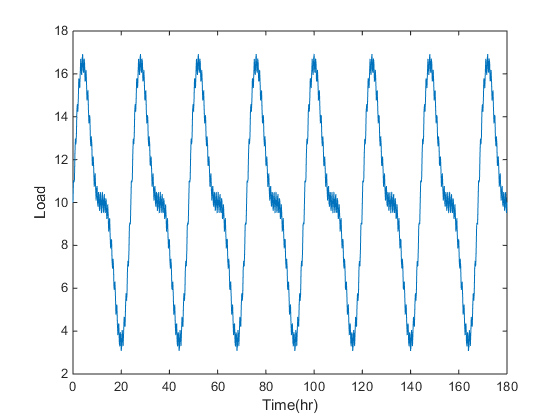
\includegraphics{CBE660_Assign8_3_Fig2.png} \\
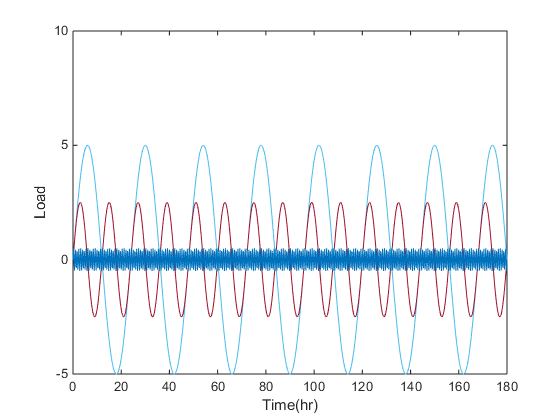
\includegraphics{CBE660_Assign8_3_Fig1.png}

\lstinputlisting{CBE660_Assign8_3.m}


\newpage


\end{document}


